\documentclass[11pt]{article}

% Packages
\usepackage[utf8]{inputenc}
\usepackage[T1]{fontenc}
\usepackage{lmodern}               
\usepackage[margin=1in]{geometry}
\usepackage{tikz}                  
\usepackage{graphicx}
\usetikzlibrary{positioning, shapes, backgrounds, matrix}
\usepackage{enumitem}
\usepackage{caption}
\usepackage{xcolor}
\pagestyle{empty}


% Colors
\definecolor{darkbg}{HTML}{1E1E1E}        
\definecolor{tealish}{HTML}{008080}    
\definecolor{textgray}{HTML}{DDDDDD}      
\definecolor{boxbg}{HTML}{2C2C2C}        
\definecolor{transportationcol}{HTML}{FF6B6B}     
\definecolor{energy/infrastructurecol}{HTML}{FFD93D}    
\definecolor{businesscol}{HTML}{6BCB77}   
\definecolor{healthcarecol}{HTML}{4D96FF}       


\usepackage[sfdefault]{FiraSans}   
\renewcommand{\familydefault}{\sfdefault}


\begin{document}
% PAGE 1

\begin{tikzpicture}[remember picture,overlay]
  \fill[tealish] (current page.north west) rectangle ([yshift=-7cm]current page.north east);
\end{tikzpicture}




\begin{tikzpicture}[remember picture,overlay]
  \node[anchor=west, text=white] at ([xshift=1.5cm,yshift=-4.0cm]current page.north west) {%
    \begin{minipage}{0.62\paperwidth}
      \raggedright
      \fontsize{40}{44}\selectfont\bfseries CATASTROPHIC\\SOFTWARE\\FAILURES\\[6pt]
      \fontsize{18}{22}\selectfont Project Team Overview
    \end{minipage}
  };
\end{tikzpicture}


\begin{tikzpicture}[remember picture,overlay]
  \node[anchor=south east, text=white, font=\small] 
    at ([xshift=-1cm,yshift=-6.5cm]current page.north east) 
    {Created by Coutinho \& Bolcau};
\end{tikzpicture}



\vspace*{3.5cm}


\begin{tikzpicture}[remember picture, overlay]
\fill[darkbg] ([yshift=-7cm]current page.north west) rectangle (current page.south east);
\end{tikzpicture}

\vspace{0.1cm}


\vspace{0.1cm}

\begin{center}
\color{textgray}
\begin{tabular}{|p{0.22\linewidth}|p{0.22\linewidth}|p{0.22\linewidth}|p{0.22\linewidth}|}
\hline
\textbf{Team Leaders} & \textbf{Git Leader} & \textbf{Git Co-Leader} & \textbf{CSS Leaders} \\
\hline
Bolcau, Çitaku & Wilinski & Bertolini & Chatterjee, Brinjevec \\
\hline
\end{tabular}
\end{center}







\vspace{0.1cm}


\begin{center}
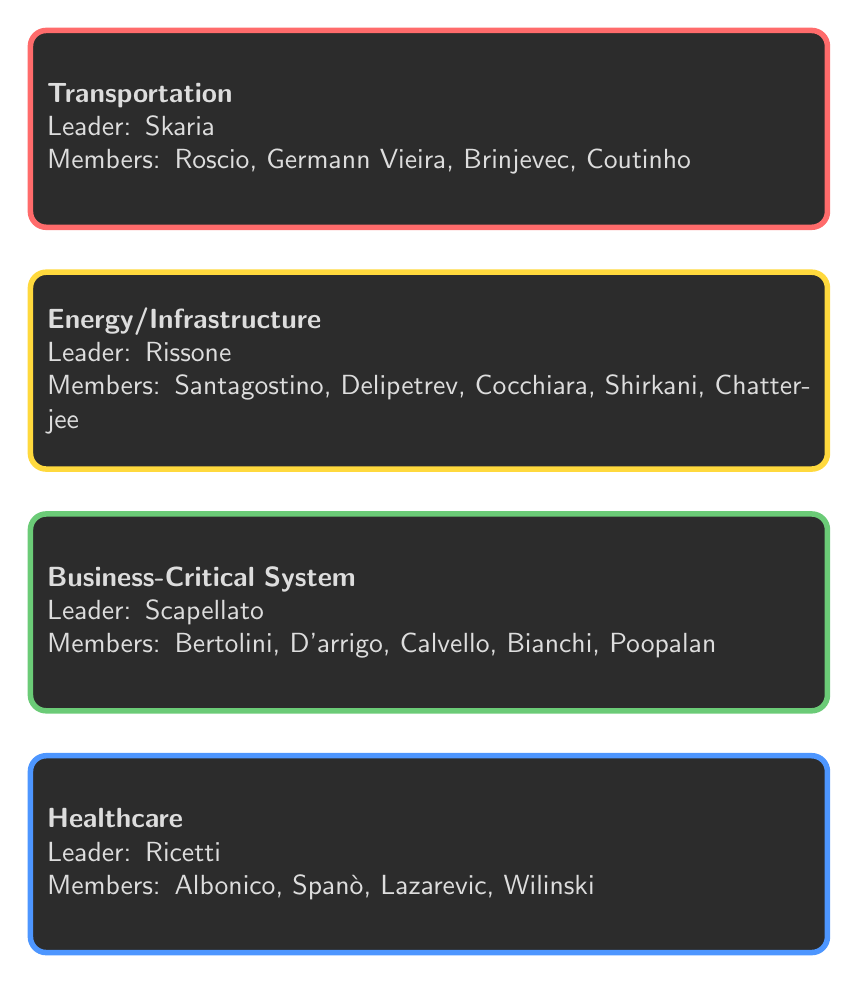
\begin{tikzpicture}[every node/.style={rectangle, rounded corners=2mm, text width=0.8\linewidth, minimum height=2.5cm, inner sep=6pt, fill=boxbg, text=textgray}]
\node[draw, line width=2pt, draw=transportationcol] (transportation) {
\textbf{Transportation} \\ Leader: Skaria \\ Members: Roscio, Germann Vieira, Brinjevec, Coutinho
};
\node[draw, line width=2pt, draw=energy/infrastructurecol, below=0.5cm of transportation] (energy/infrastructure) {
\textbf{Energy/Infrastructure} \\ Leader: Rissone \\ Members: Santagostino, Delipetrev, Cocchiara, Shirkani, Chatterjee 
};
\node[draw, line width=2pt, draw=businesscol, below=0.5cm of energy/infrastructure] (business) {
\textbf{Business-Critical System} \\ Leader: Scapellato \\ Members: Bertolini, D'arrigo, Calvello, Bianchi, Poopalan
};
\node[draw, line width=2pt, draw=healthcarecol, below=0.5cm of business] (healthcare) {
\textbf{Healthcare} \\ Leader: Ricetti \\ Members: Albonico, Spanò, Lazarevic, Wilinski
};
\end{tikzpicture}
\end{center}



\newpage


% PAGE 2 


\begin{tikzpicture}[remember picture, overlay]
  \fill[darkbg] (current page.north west) rectangle (current page.south east);
\end{tikzpicture}


\begin{center}
     {\fontsize{28}{32}\selectfont\bfseries\color{white} Topics Summary}
\end{center}


\vspace*{0.5cm} 


\begin{center}
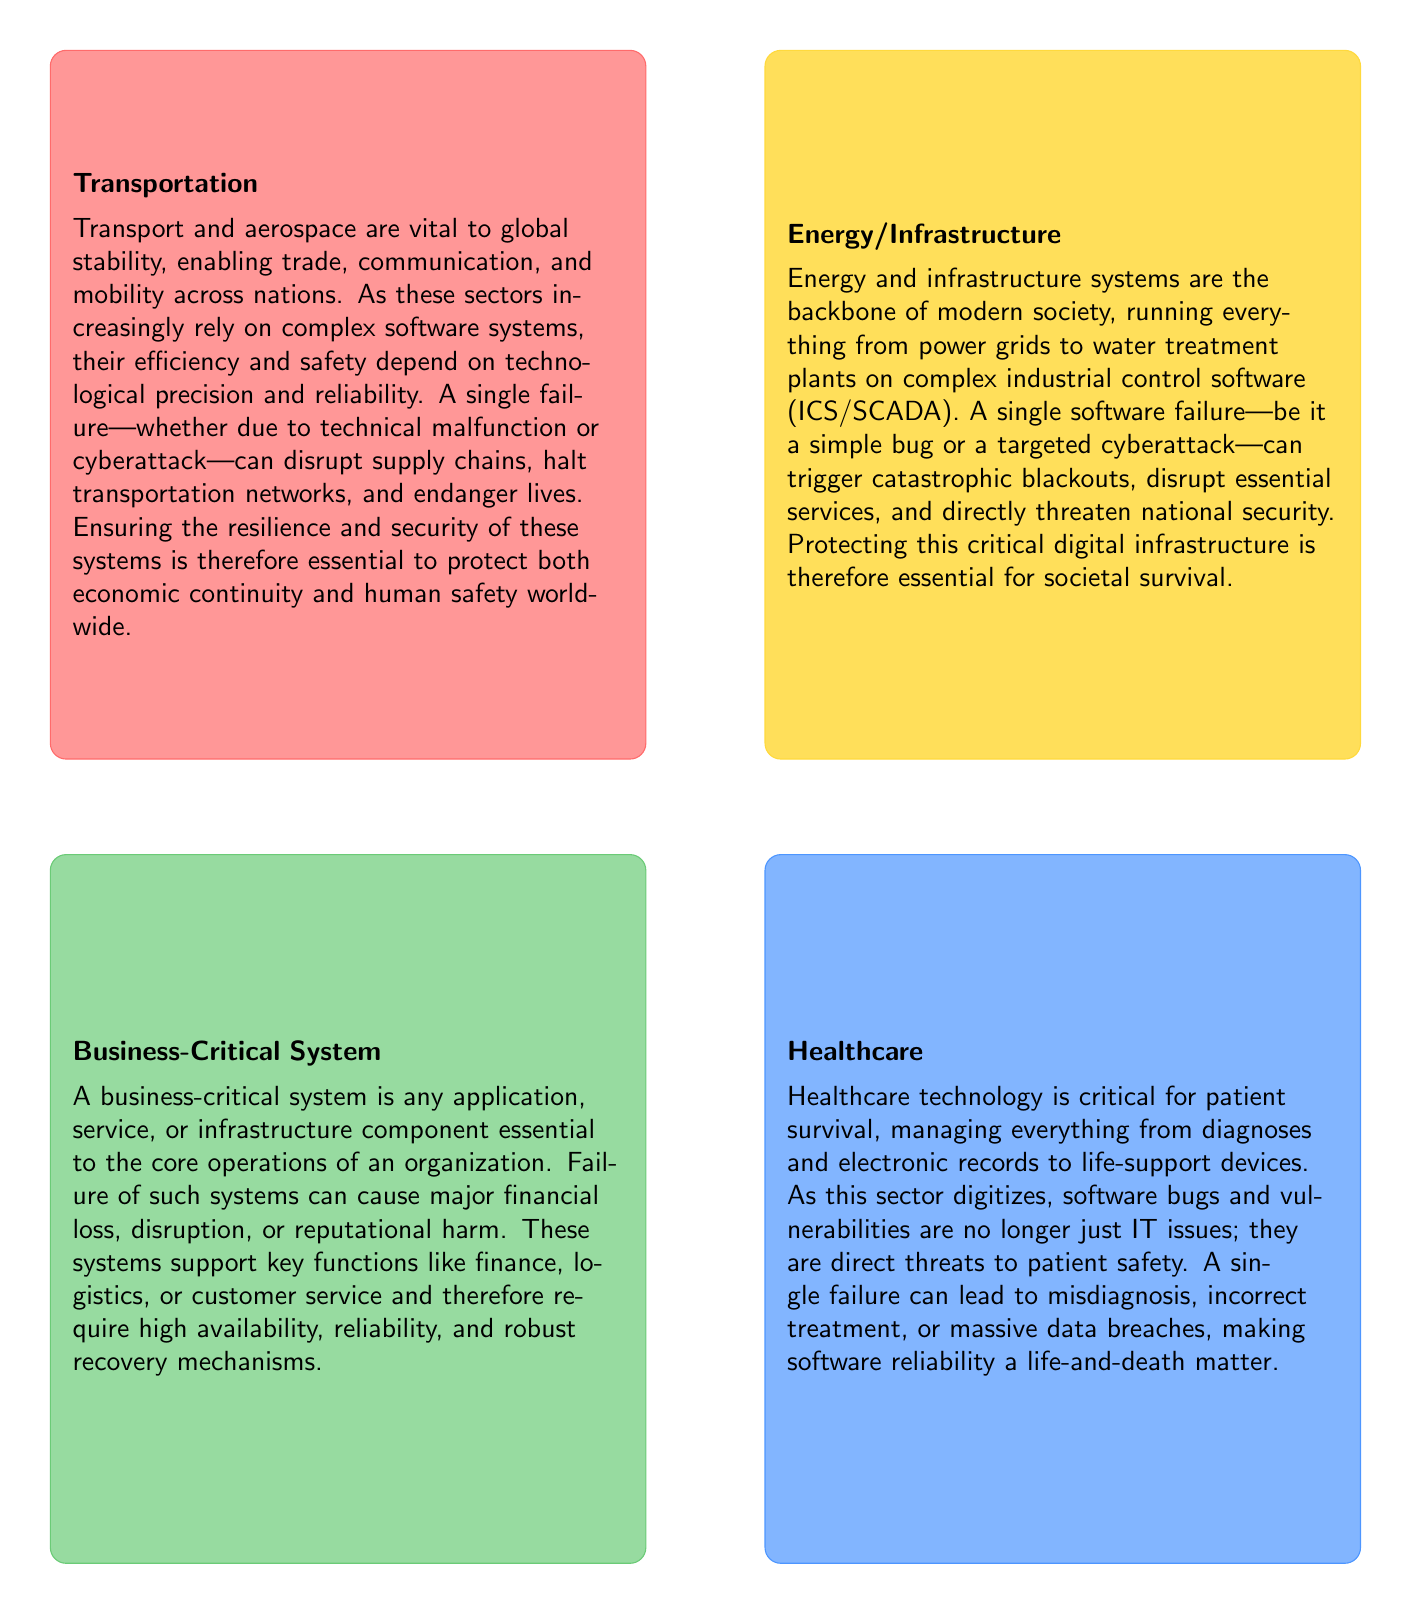
\begin{tikzpicture}[every node/.style={inner sep=8pt, align=left}]
\matrix[column sep=1.5cm, row sep=1.2cm,
  nodes={draw, rounded corners=2mm, text width=7cm, minimum height=9cm, inner sep=8pt, text=white
  }, anchor=north] (m) {

% Row 1
\node[fill=transportationcol!70, draw=transportationcol] (transportation) {
\textbf{\textcolor{black}{Transportation}}\\[4pt]
\textcolor{black}{Transport and aerospace are vital to global stability, enabling trade, communication, and mobility across nations. As these sectors increasingly rely on complex software systems, their efficiency and safety depend on technological precision and reliability.
A single failure—whether due to technical malfunction or cyberattack—can disrupt supply chains, halt transportation networks, and endanger lives. Ensuring the resilience and security of these systems is therefore essential to protect both economic continuity and human safety worldwide.}
}; &

\node[fill=energy/infrastructurecol!85, draw=energy/infrastructurecol] (Energy/infrastructure) {
\textbf{\textcolor{black}{Energy/Infrastructure}}\\[4pt]
\textcolor{black}{Energy and infrastructure systems are the backbone of modern society, running everything from power grids to water treatment plants on complex industrial control software (ICS/SCADA).
A single software failure—be it a simple bug or a targeted cyberattack—can trigger catastrophic blackouts, disrupt essential services, and directly threaten national security. Protecting this critical digital infrastructure is therefore essential for societal survival.}
}; \\

% Row 2
\node[fill=businesscol!70, draw=businesscol] (business) {
\textbf{\textcolor{black}{Business-Critical System}}\\[4pt]
\textcolor{black}{A business-critical system is any application, service, or infrastructure component essential to the core operations of an organization. Failure of such systems can cause major financial loss, disruption, or reputational harm. These systems support key functions like finance, logistics, or customer service and therefore require high availability, reliability, and robust recovery mechanisms.
}
}; &

\node[fill=healthcarecol!70, draw=healthcarecol] (healthcare) {
\textbf{\textcolor{black}{Healthcare}}\\[4pt]
\textcolor{black}{Healthcare technology is critical for patient survival, managing everything from diagnoses and electronic records to life-support devices.
As this sector digitizes, software bugs and vulnerabilities are no longer just IT issues; they are direct threats to patient safety. A single failure can lead to misdiagnosis, incorrect treatment, or massive data breaches, making software reliability a life-and-death matter.
}
}; \\
};
\end{tikzpicture}
\end{center}


\newpage
\begin{tikzpicture}[remember picture, overlay]
  \fill[darkbg] (current page.north west) rectangle (current page.south east);
\end{tikzpicture}
\vspace*{\fill}
\begin{center}
     {\fontsize{28}{32}\selectfont\bfseries\color{white} Repository tree}
\end{center}
\vspace{1cm}
\begin{figure}[h!]
    \centering
    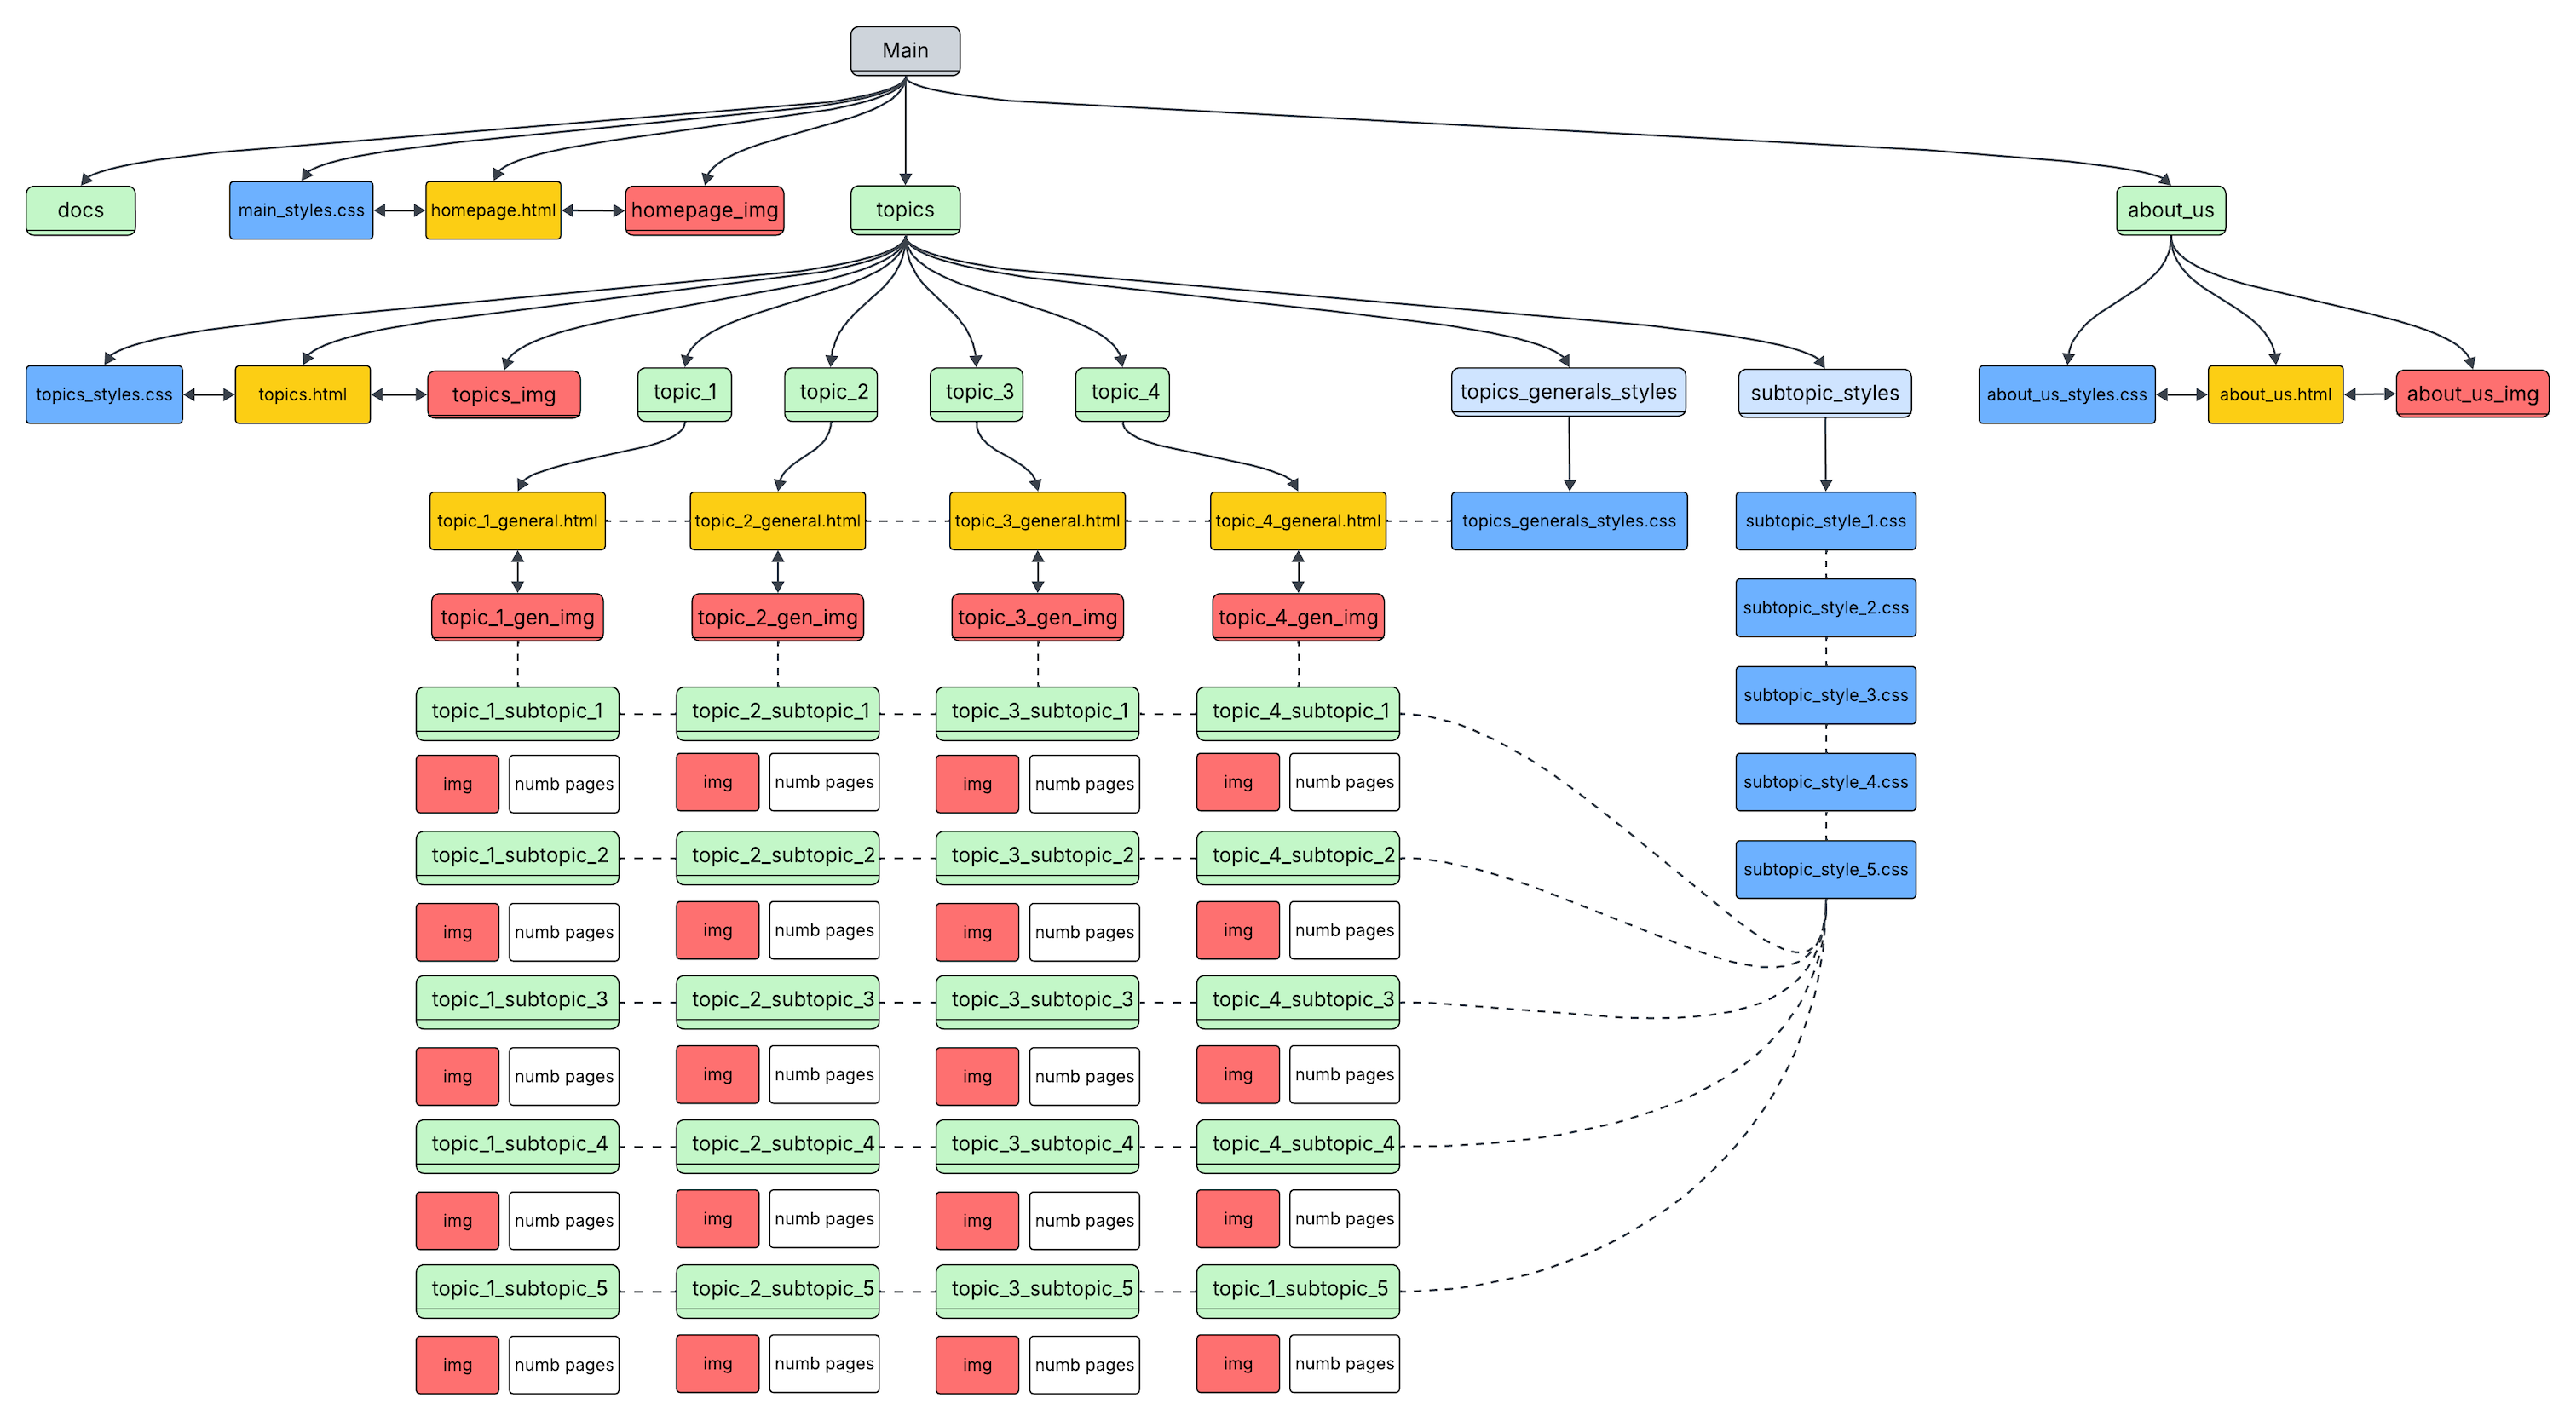
\includegraphics[width=1\textwidth]{inception_images/repo_three.png} 
\end{figure}
\vspace*{\fill}

\newpage
\begin{tikzpicture}[remember picture, overlay]
  \fill[darkbg] (current page.north west) rectangle (current page.south east);
\end{tikzpicture}
\vspace*{\fill} 
\begin{center}
     {\fontsize{28}{32}\selectfont\bfseries\color{white} Organization}
\end{center}
\vspace{0.3cm}
\textcolor{white}{In our organization, the Discord server is essential. As shown in figure, 
we have a well-defined channel structure (on the left) and a role system (on the right).}
\vspace{0.3cm}
\begin{center}
\begin{tikzpicture}
\node[inner sep=0] (img1) at (0,0) {
    
\includegraphics[width=0.3\textwidth]{inception_images/server.png}
};
\node[inner sep=0] (img2) at ([xshift=7cm]img1.east) {  % Adjust 8cm based on your needs
    
\includegraphics[width=0.6\textwidth]{inception_images/roles.png}
};
\end{tikzpicture}
\end{center}
\vspace*{\fill} 

\newpage
\begin{tikzpicture}[remember picture, overlay]
  \fill[darkbg] (current page.north west) rectangle (current page.south east);
\end{tikzpicture}
\vspace*{\fill}
\begin{center}
  {\fontsize{32}{38}\selectfont\bfseries\color{white} Of course, no project is complete\\[0.3cm] without \textit{ambitious} deadlines... }\end{center}
\vspace*{\fill}

\newpage
\begin{tikzpicture}[remember picture, overlay]
  \fill[darkbg] (current page.north west) rectangle (current page.south east);
\end{tikzpicture}
\vspace*{\fill}
\begin{center}
     {\fontsize{28}{32}\selectfont\bfseries\color{white} Project Timeline}
\end{center}
\vspace{1cm}
\begin{figure}[h!]
    \centering
    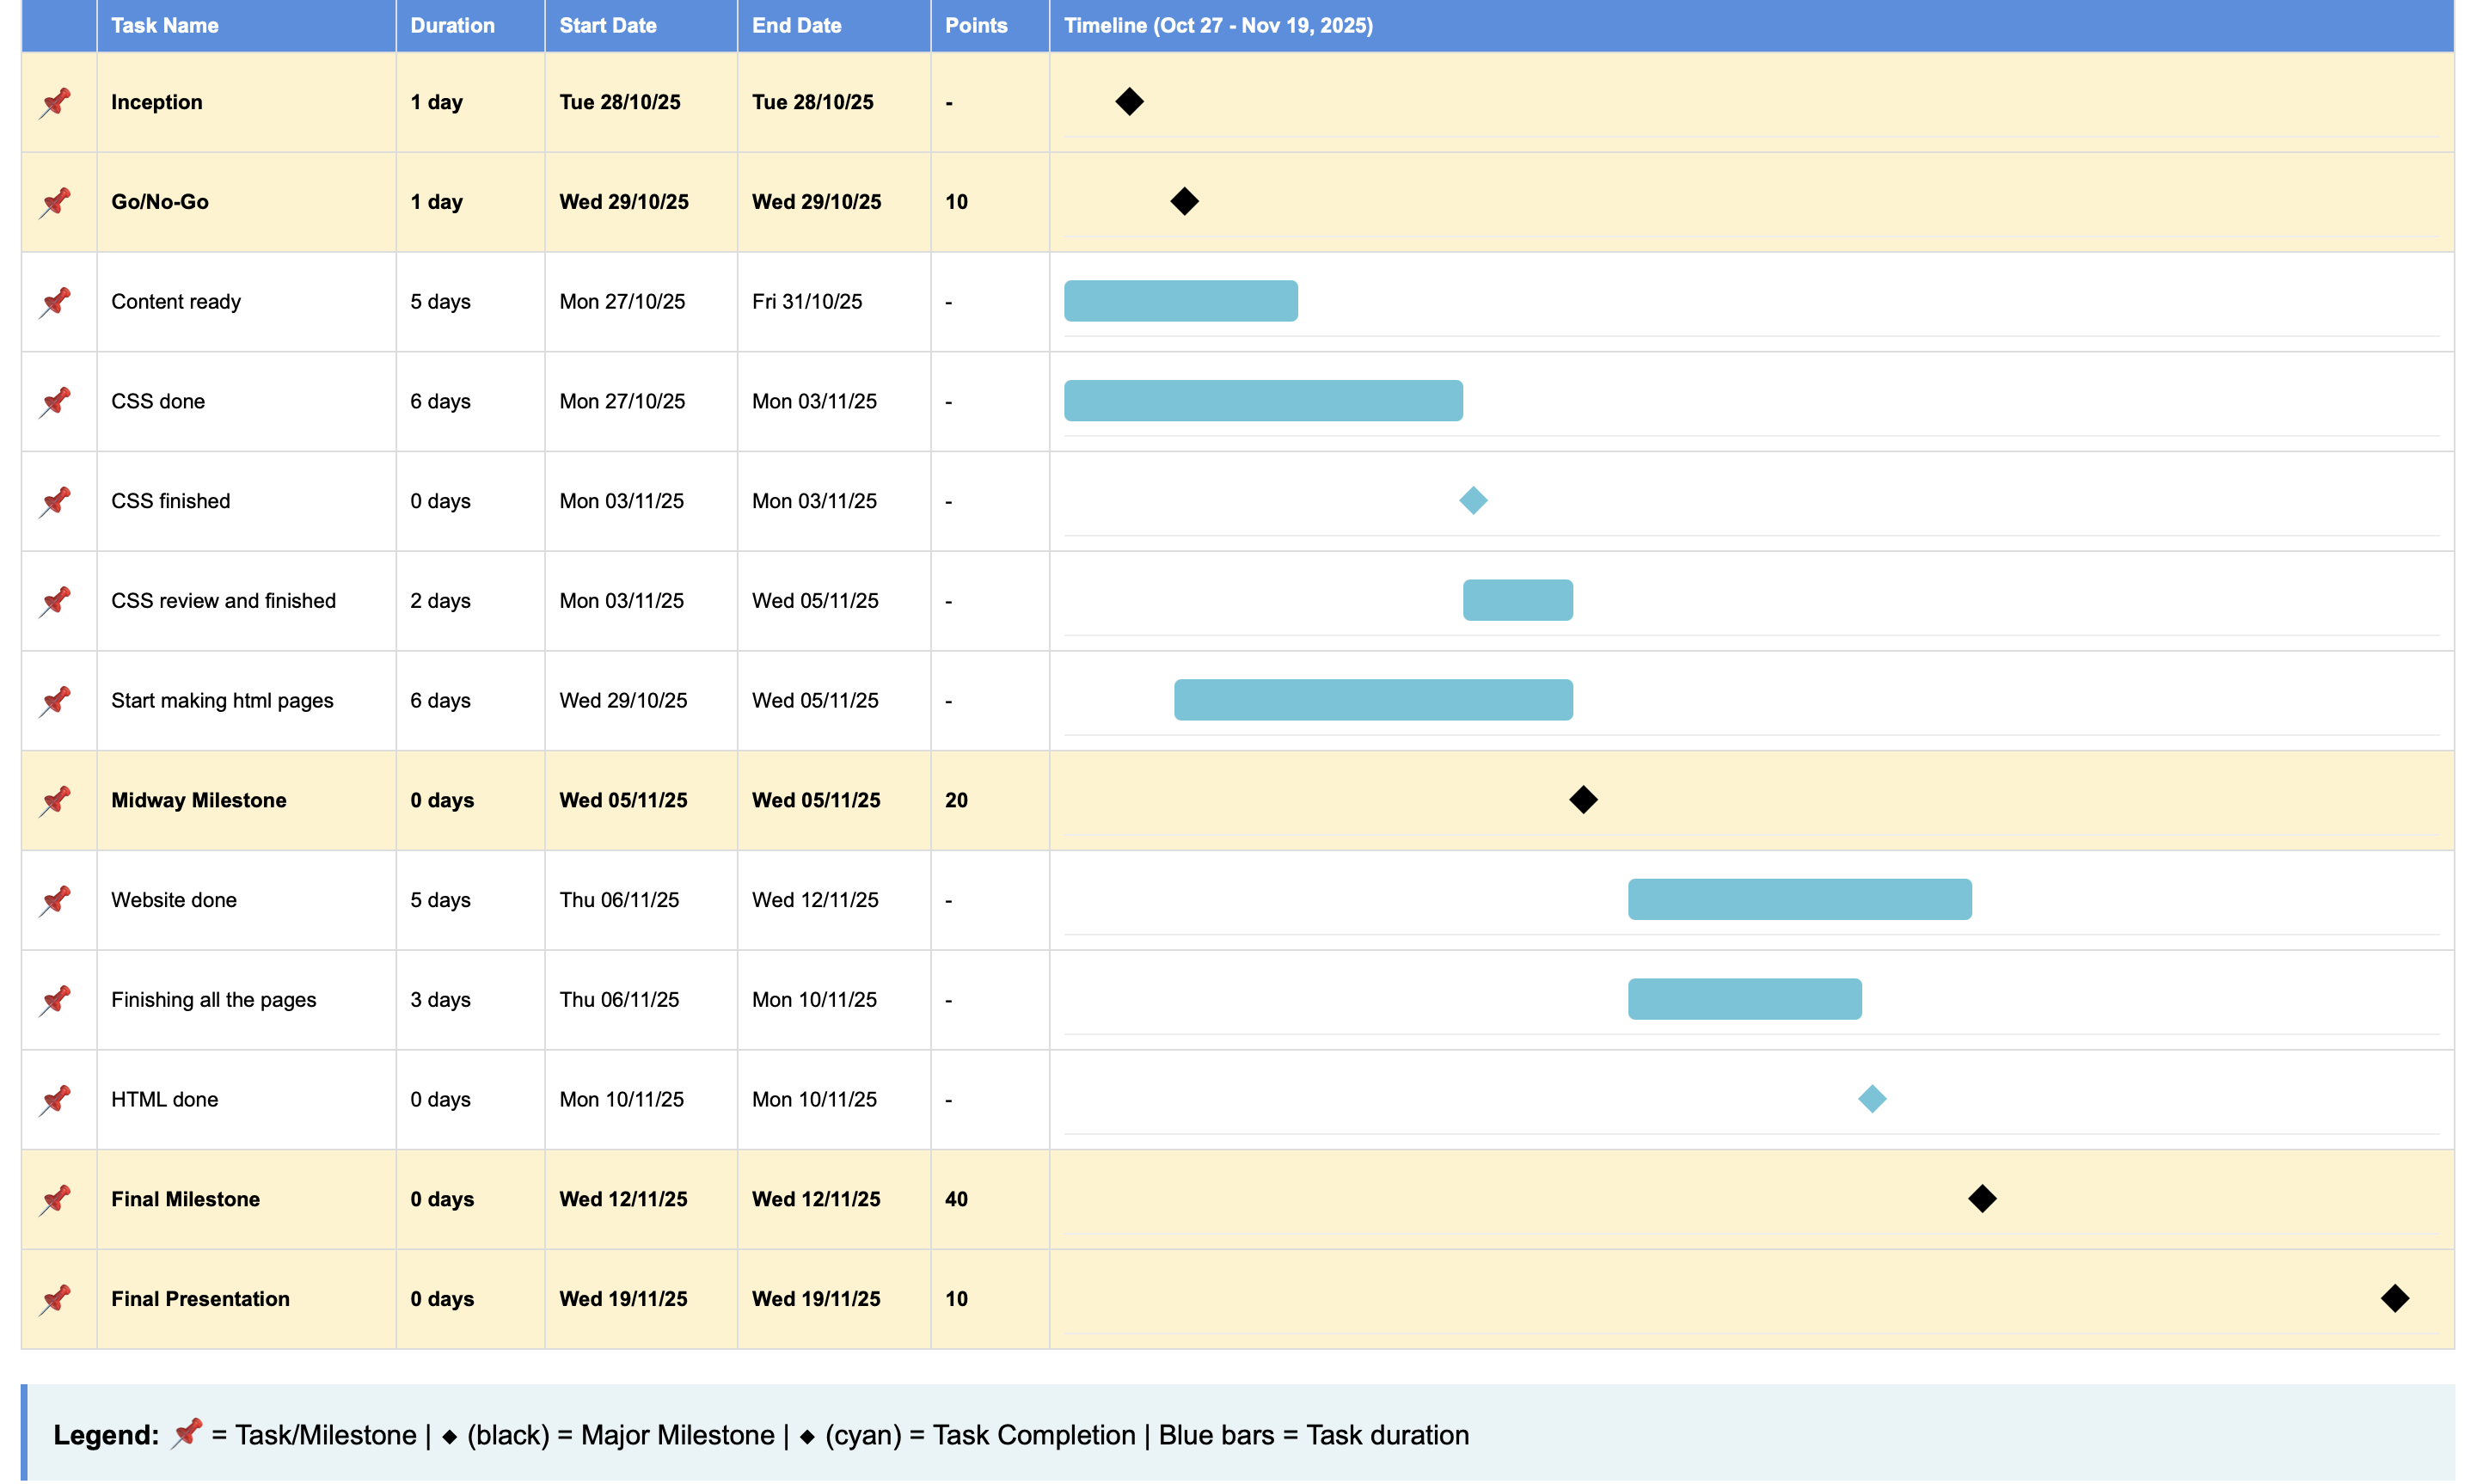
\includegraphics[width=0.95\textwidth]{inception_images/gantt.png} 
\end{figure}
\vspace*{\fill}
\end{document}
